\documentclass{beamer}
\usepackage[english]{babel}
\usepackage[latin1]{inputenc}
\usepackage{enumerate}
\usepackage{amsmath}
\usepackage{graphicx}
\usepackage{tikz}
\usepackage{subfigure}
\usetheme{Warsaw}

\AtBeginSection[]
{
  \begin{frame}
    \frametitle{Table of Contents}
    \tableofcontents[currentsection]
  \end{frame}
}

\begin{document}
\title{Designing a dynamic kick for a Nao robot}
\author{Inge Becht \\ Maarten de Jonge \\ Richard Pronk}
\institute{University of Amsterdam}
\date{\today}


\begin{frame}
  \titlepage
\end{frame}

\section{Goal}
\begin{frame}{Goal}
  \begin{itemize}
    \item Creating a dynamic kick instead of a key-frame motion
    \item Handle external forces without falling
  \end{itemize}
  \pause
  Benefits:
  \begin{itemize}
    \item more stable
    \item omni-directional
    \item potentially harder
    \item supporting the Dutch Nao Team
  \end{itemize}
\end{frame}

\section{About Nao}
\begin{frame}{About Nao}
\begin{columns}[T]
    \begin{column}{.5\textwidth}
	\vspace{20 mm}
	\begin{itemize}
		\item Aldebaran Robotics
        \item Used in RoboCup SPL
	   	\item 8 force sensitive resistors
		\item The coordinate space
	\end{itemize}	
    \end{column}
    \begin{column}{.5\textwidth}

% Your image included here
    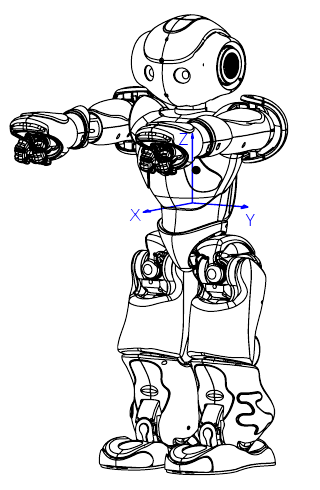
\includegraphics[scale=0.5]{pics/hardware_inertialunit.png}

    \end{column}
  \end{columns}
\end{frame}

\section{Balancing}
\begin{frame}{Balancing}
  Two components:
  \begin{itemize}
    \item staying balanced during kick trajectory
    \item react to external forces
  \end{itemize}
\end{frame}

\begin{frame}{Proportional-integral-derivative controller}
  Both components use a variant of the PID controller:
  \begin{align*}
    out(t) = K_p e(t) + K_i \int_{0}^{t} e(\tau) d\tau + K_d \frac{d}{dt} e(t)
  \end{align*}
\end{frame}

\begin{frame}{Stripping it down}
  PD- and P-controller:
  \begin{align*}
    out(t) &= K_p e(t) + K_d \frac{d}{dt} e(t) \\
    out(t) &= K_p e(t)
  \end{align*}
\end{frame}

\subsection{Center of Mass Controller}
\begin{frame}{Center of Mass}
  \begin{block}{Balance}
    A humanoid body is balanced when the projection of its center of
mass unto the ground lies within its support polygon
  \end{block}
  Center of mass:
  \begin{align*}
    \frac{\sum_i \vec{c}_i m_i}{M}
  \end{align*}
  Support polygon:
  \begin{itemize}
    \item the convex hull of the contact points with the ground
    \item in case of a robot standing on one leg: the center of its foot
  \end{itemize}
\end{frame}

\begin{frame}{P-Controller}
  \begin{itemize}
    \item CoM calculated through forward kinematics
    \item Uses a simple P-Controller
    \begin{itemize}
      \item separate for the forwards and sideways directions
    \end{itemize}
    \item Actuation in ankle pitch and roll
  \end{itemize}
\end{frame}

\subsection{Using the force sensitive resistors}
\begin{frame}{Grouping the sensors}
\begin{figure}[htb]
	\centering
	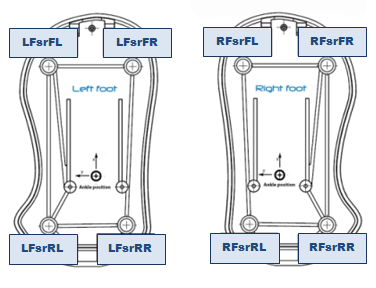
\includegraphics[scale=0.45]{pics/naosfeet.jpg}
	\label{fig:fsr_plot}
\end{figure}
\begin{itemize}
    \item $Front_t = (1-s) * Front_{t-1} + s * (LFsrFL + LFsrFR)$
    \item $Left_t = (1-s) * Left_{t-1} + s *(LFsrFL + LFsrRL)$
    \item $Right_t = (1-s) * Right_{t-1} + s *(LFsrFR + LFsrRR)$
    \item $Back_t = (1-s) * Back_{t-1} + s *(LFsrRL + LFsrRR)$ 
\end{itemize}
\end{frame}

\begin{frame}{Using a PD controller to calculate the angle offsets}
Error is calculated by:
\begin{itemize}
    \item $e(t)_x = (Front_t - Back_t)$
    \item $e(t)_y = (Right_t - Left_t)$
\end{itemize}
The PD controller:
\begin{itemize}
    \item $P_{out} x = e(t)_xK_p$
    \item $P_{out} y = e(t)_yK_p$
    \item $D_{out} x = \frac{e(t)_x - e(t-1)_x}{timeTaken}K_d$
    \item $D_{out} y = \frac{e(t)_y - e(t-1)_y}{timeTaken}K_d$
\end{itemize}
The angle offsets:
\begin{itemize}
    \item  $Offset$ $Hip$ $Pitch$ $= P_{out}x + D_{out}x$ 
    \item $Offset$ $Hip$ $Roll$ $=  P_{out}y + D_{out}y$ 
\end{itemize}
\end{frame}

\begin{frame}{Error band}
\begin{itemize} 
   \item Allows conversion
   \item Less overshoot
   \item Smaller chance of oscillation
\end{itemize}
\vspace{10 mm}
\[
  P_{out}x = \left\{ 
  \begin{array}{l l}
     e(t)_xK_p& \quad \text{if $e(t)_x < Thres_{min X}$ or $e(t)_x > Thres_{max X}$}\\ 
     0& \quad \text{Otherwise}\\
  \end{array} \right.
\]
\vspace{2 mm}
same for $P_{out}y$, $D_{out}x$ and $D_{out}y$.
\end{frame}

\begin{frame}
\centering
 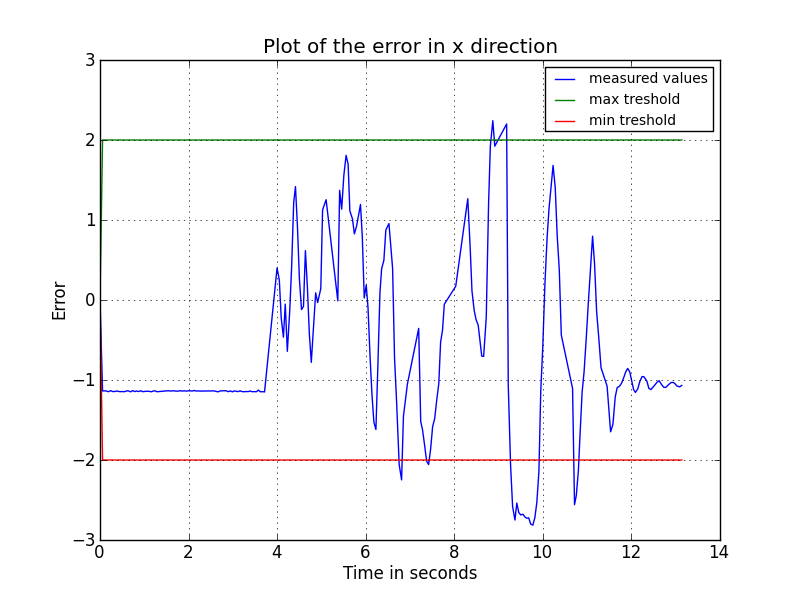
\includegraphics[scale=0.5]{pics/back_balanceon_X.png}
\end{frame}

\begin{frame}{Sampling rate issues}
Sampling rate is determined by the CPU power availability.
Parameters are dependent on the sampling rate. 
\vspace{5 mm}
\begin{itemize}
	\item $Offset$ $Hip$ $Pitch$ $= (P_{out}x + D_{out}x) * timeTaken $ 
	\item $Offset$ $Hip$ $Roll$ $=  (P_{out}y + D_{out}y) * timeTaken$ 
\end{itemize}
\vspace{5 mm}
As timeTaken increases so does the angle offsets in a linear way.
\end{frame}



\begin{frame}{Startup error}
\begin{itemize}
\item Big sample rate differences during startup
\item Low pass filter
\vspace{5 mm}
\end{itemize}
\footnotesize
\[
  Offset Hip Pitch = \left\{ 
  \begin{array}{l l}
     (P_{out}x + D_{out}x) * timeTaken& \quad \text{if $\nabla TimeTaken < Thres_{low-pass}$}\\ 
    0 & \quad \text{Otherwise}\\
  \end{array} \right.
\]

\[
  Offset Hip Roll = \left\{ 
  \begin{array}{l l}
     (P_{out}y + D_{out}y) * timeTaken& \quad \text{if $\nabla TimeTaken < Thres_{low-pass}$}\\ 
    0 & \quad \text{Otherwise}\\
  \end{array} \right.
\]
\normalsize
\end{frame}

\begin{frame}{Movie}

\end{frame}

\section{Inverse Kinematics}
\begin{frame}{Introduction}
  Forward kinematics: Given a set of joint angles, where are the end effectors?
  
  Inverse kinematics: Given desired locations for the end effectors, what is the
  corresponding set of joint angles?
\end{frame}

\begin{frame}{Terminology}
  Let:
  \begin{itemize}
  \item $\theta$ be a $1 \times n$ vector describing the angles of $n$ joints
  \item $\vec{t}$ the vector containing the goal position for each end effector
  \item $\vec{s}$ the vector of the end effectors' current positions
  \item $\vec{e} = \vec{t} - \vec{s}$
  \end{itemize}
\end{frame}

\begin{frame}{Forwards and backwards}
  Viewing end effector locations as a function of the joint angles, we want:
  \begin{align*}
    \vec{t} = \vec{s}(\theta)
  \end{align*}

  \begin{itemize}
    \item not always solvable
    \item can be approached iteratively
  \end{itemize}
\end{frame}

\begin{frame}{Linear approximation}
  \begin{itemize}
  \item Use the first-order derivative of the end effector locations with
    respect to the joint angles as a linear approximation
  \item known as the \emph{Jacobian}
  \end{itemize}
  \begin{block}{The Jacobian}
    \begin{align*}
      J(\theta)_{i, j} &= \frac{\partial s_i}{\partial \theta_j} \\
      \frac{\partial s_i}{\partial \theta_j} &= v_j \times (s_i - p_j)
    \end{align*}
  \end{block}
\end{frame}

\begin{frame}{Iterative solution}
  Linear approximation:
  \begin{align*}
    \Delta \vec{s} = J \Delta\theta
  \end{align*}
  We're interested in:
  \begin{align*}
    \vec{e} = J \Delta\theta
  \end{align*}
  and thus:
  \begin{align*}
    \Delta \theta = J^{-1} \vec{e}
  \end{align*}
  \pause
  Because it's only a linear approximation, place an upper limit on the length
  of $\vec{e}$.
\end{frame}

\begin{frame}{Inverting the Jacobian}
  \begin{itemize}
    \item Jacobian usually can't be inverted
    \item In our case: $3\times4$ matrix
  \end{itemize}
  \pause
  Three common methods of approximating the inverse:
  \begin{itemize}
    \item Jacobian transpose: $J^{-1} \approx \alpha J^T$
    \item Moore-Penrose pseudo-inverse: $J^{-1} \approx J^{+}$
    \item Damped Least Squares: $(J^T J  + \lambda^2 I)^1 J^T$
  \end{itemize}
\end{frame}

\section{Trajectory Planning}
\begin{frame}{The different stages of a kick}
    A kick consists of multiple stages
    \begin{itemize}
        \item Initial Pose
        \item Contact Point
        \item Retraction Point
    \end{itemize}
    We assume that ball position is given relative to the foot and the direction
    is given as a position in space.
\end{frame}

\begin{frame}{Initial Pose}
    \begin{itemize}
        \item The first step in making a kick
        \item normalPose in which the center of mass balancer is used to find
            the most balanced position
    \end{itemize}

    \begin{figure}[htbp]
      \centering
      \makebox[\textwidth] {
        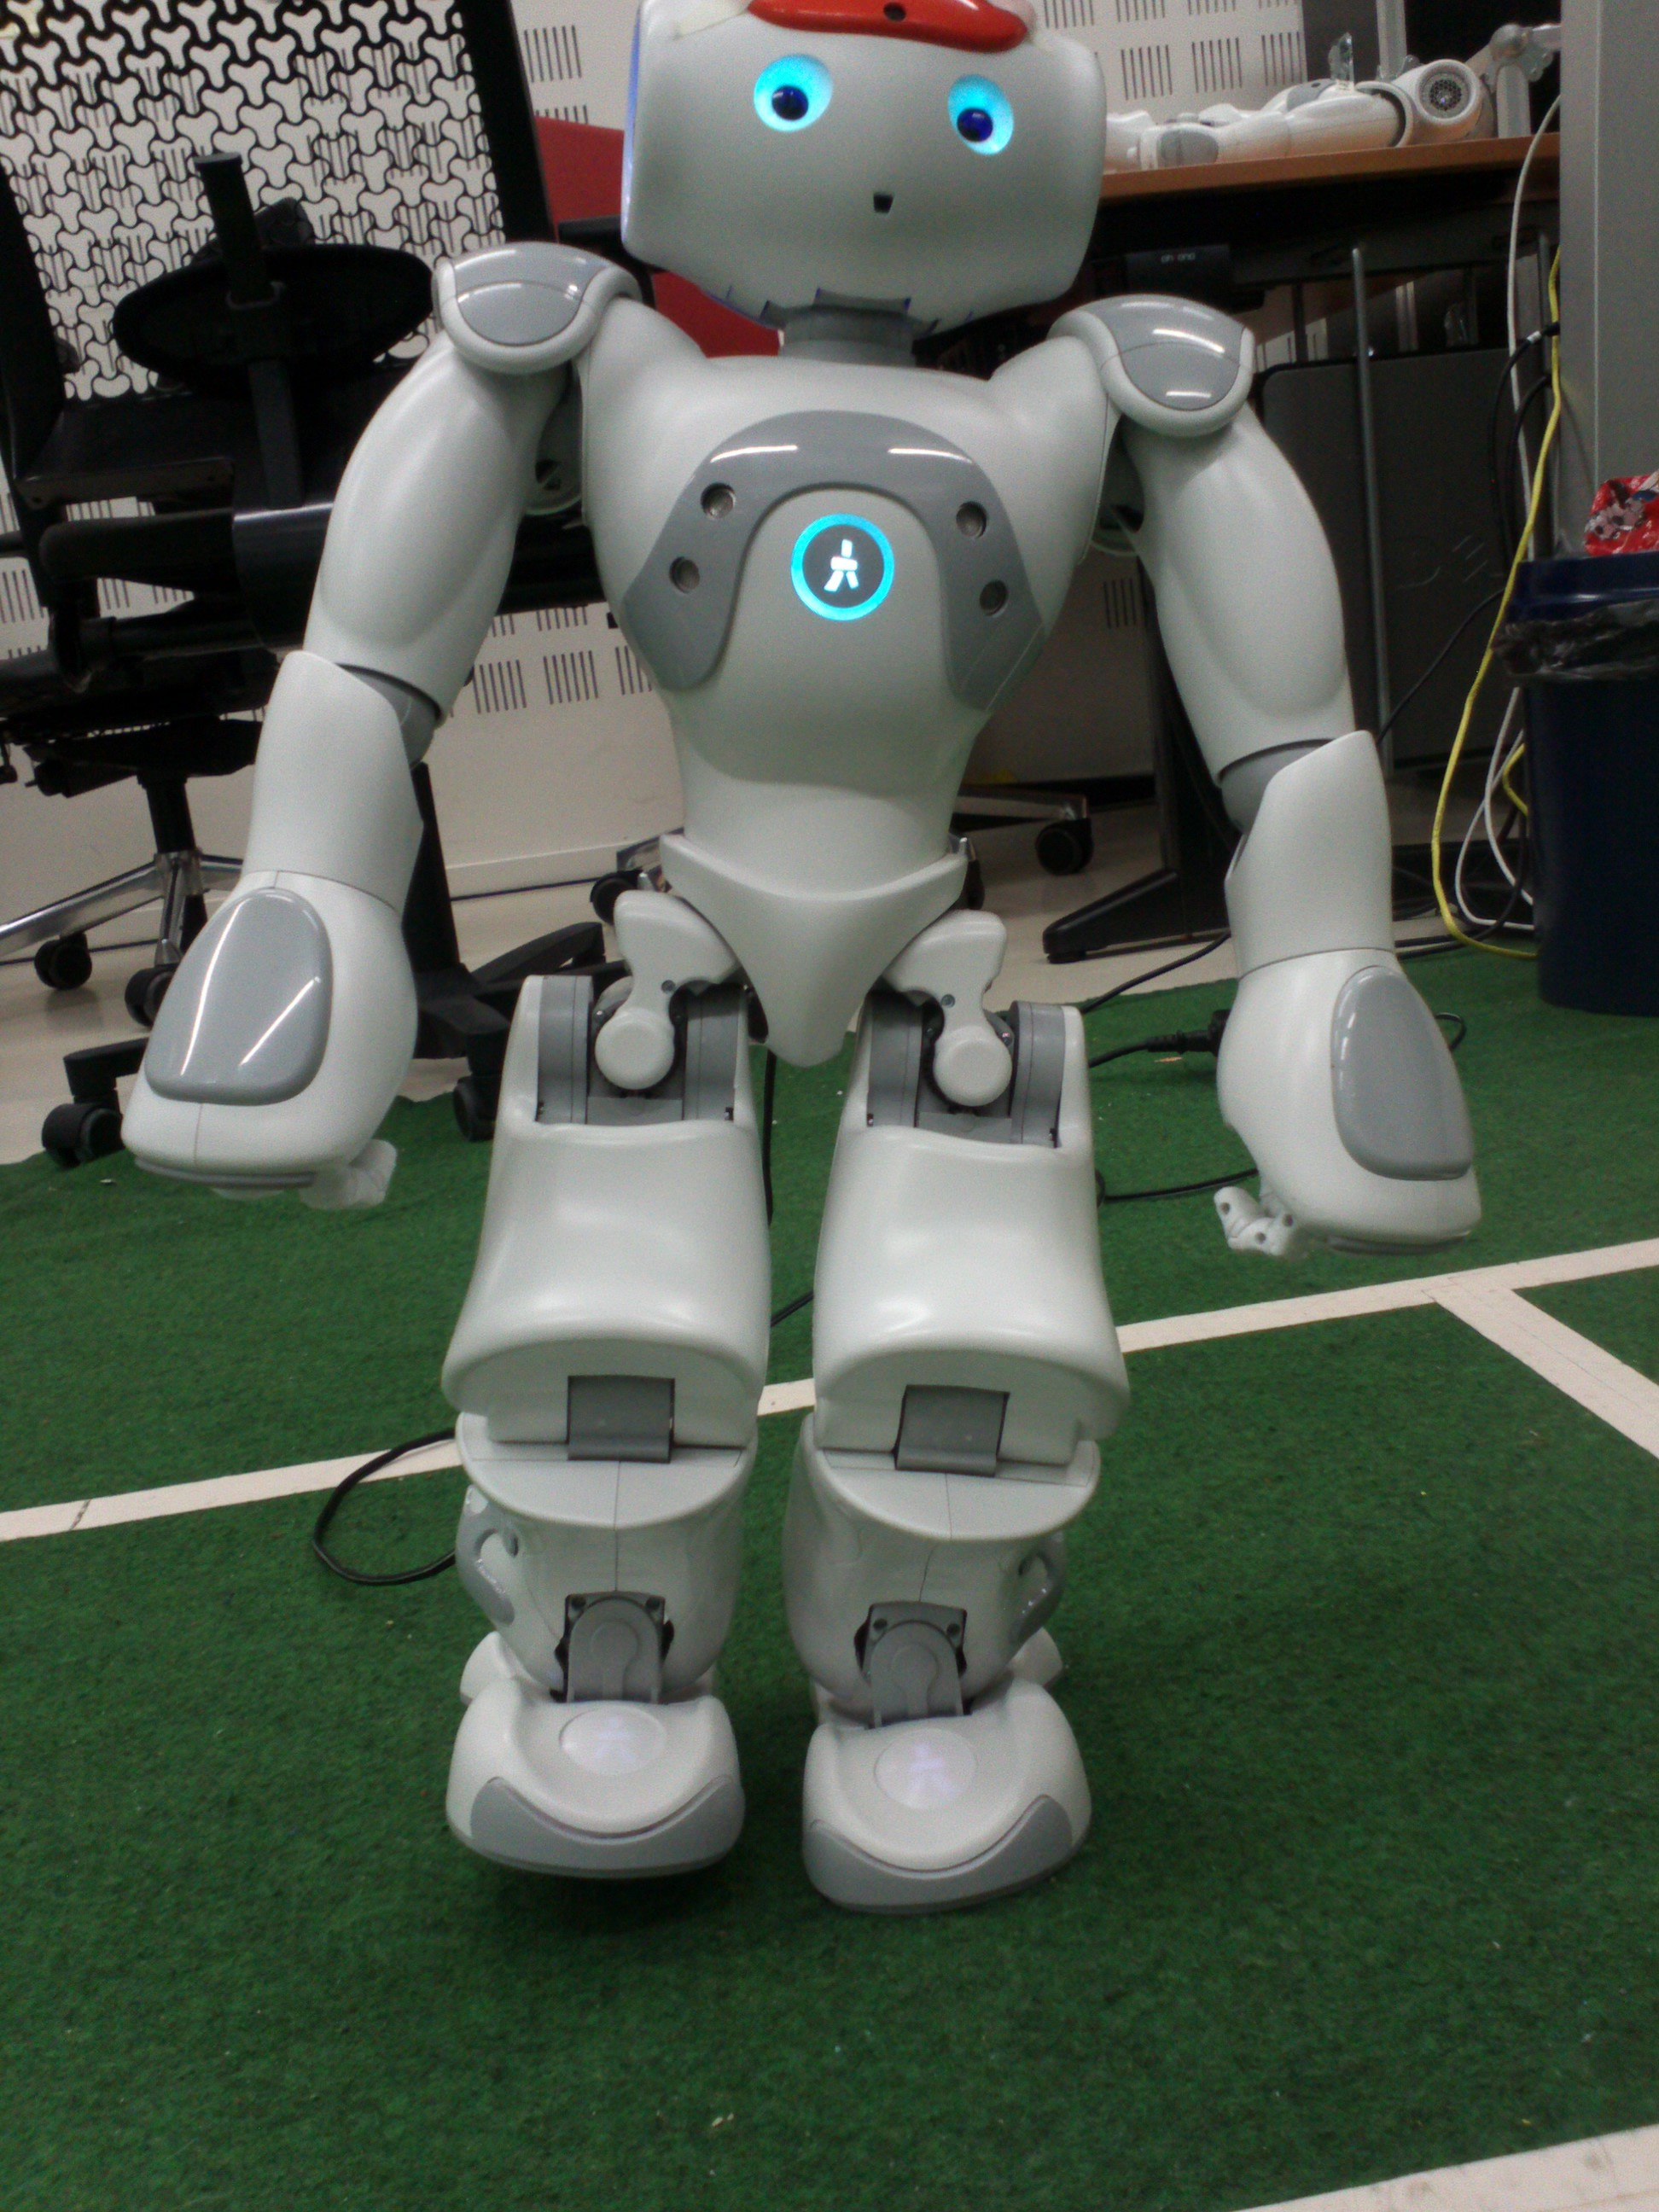
\includegraphics[width=0.3\textwidth]{pics/nao_initial2.jpg}
      }
      \caption{Initial position of the Nao with left leg as support leg.}
    \end{figure}
\end{frame}

\begin{frame}{Contact Point}
    \begin{itemize}
        \item The position in space where the foot of the Nao should hit the ball
    \end{itemize}

    \begin{align*}
        \vec{c} - ( \vec{e} * r )
    \end{align*}
\end{frame}


\begin{frame}{Retraction Point} 
    \begin{itemize}
        \item      The retraction point is the farthest point from which the kick commences.
        \item      Distance
        \item      Accuracy
    \end{itemize}
\end{frame}


\begin{frame}{Retraction Point: Calculating the distance} 
    We favour the distance the most in $x$ and $y$ direction, while keeping the
    $z$ artificially high
        \begin{align}
            d_r = \vec{e}^{x} * || \vec{p}^{x} -\vec{p}_{c}^{x}|| + \vec{e}^y *
        ||\vec{p}^{y} - \vec{p}_{c}^y|| +  ||
     \vec{p}^z - \vec{p}_{c}^z|| * 0.3
        \end{align}
\end{frame}

\begin{frame}{Retraction Point: Calculating the accuracy}
    
\begin{figure}
  \resizebox{\textwidth}{!} {
    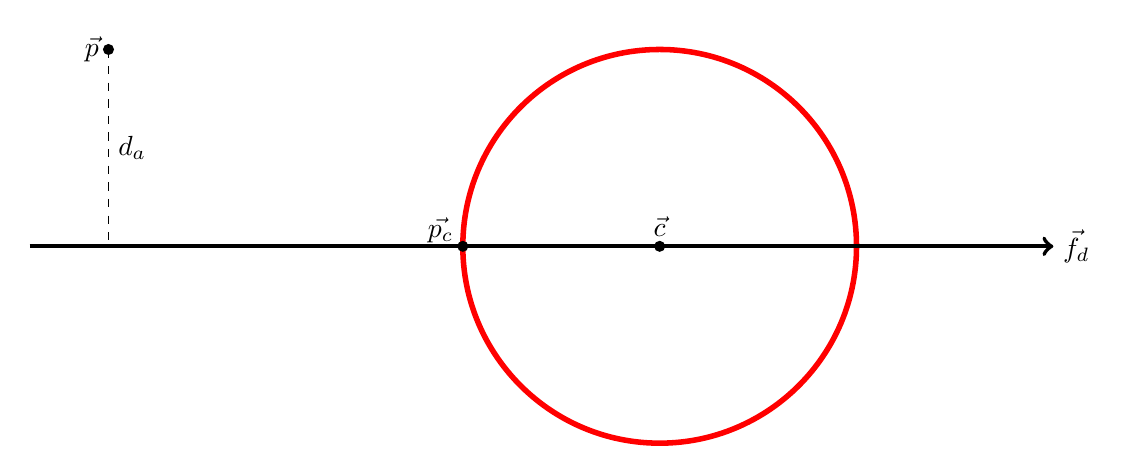
\begin{tikzpicture}
        \coordinate [label=left:$\vec{p_c}$] (A) at (-2.5,0.2);
        \coordinate [label=right:$\vec{f_d}$] (B) at (5, 0 );
        \coordinate [label=right:$d_a$] (F) at (-7, 1.25);
        \coordinate [label=above:$\vec{c}$](C) at (0,0);
        \coordinate (D) at (-2.5, 0);
        \coordinate [label=left:$\vec{p}$] (E) at (-7, 2.5);
        \draw[line width = 2][color = red] (0,0) circle (2.5cm);
        \draw [style = thick][line width = 1.5][->](-8, 0) -- (B);
        \draw[dashed] (E) -- (-7,0);
        \foreach \point in {C,D,E}
        \fill [black,opacity=1] (\point) circle (2pt);
    \end{tikzpicture}
    }
    \label{fig:accuracy}
\end{figure}    
\begin{align*}
    d_a = \frac{||(\vec{p}^{xy} -\vec{p_c}^{xy}) \times (\vec{p}^{xy} -
    \vec{f_d}^{xy})||}{\|\vec{f_d}^{xy}- \vec{p_c}^{xy}\|}
\end{align*}
\end{frame}


\begin{frame}{Retraction Point: Making the trade-off}
\begin{align*}
    \vec{p} = 1-\delta * d_r + \delta * \frac{100}{d_a}
\end{align*}

\begin{itemize}
    \item $\delta$ chosen rather high
    \item all points $\vec{p}$ are points in a range around the Naos leg in
        the initialpose. 
\end{itemize}
\end{frame}

\begin{frame}{Results}
\footnotesize{ $\vec{d} = \begin{bmatrix} 1\\ 0 \\ 0  \end{bmatrix}$}
\begin{figure}[htbp]
  \centering
  \makebox[\textwidth] {
    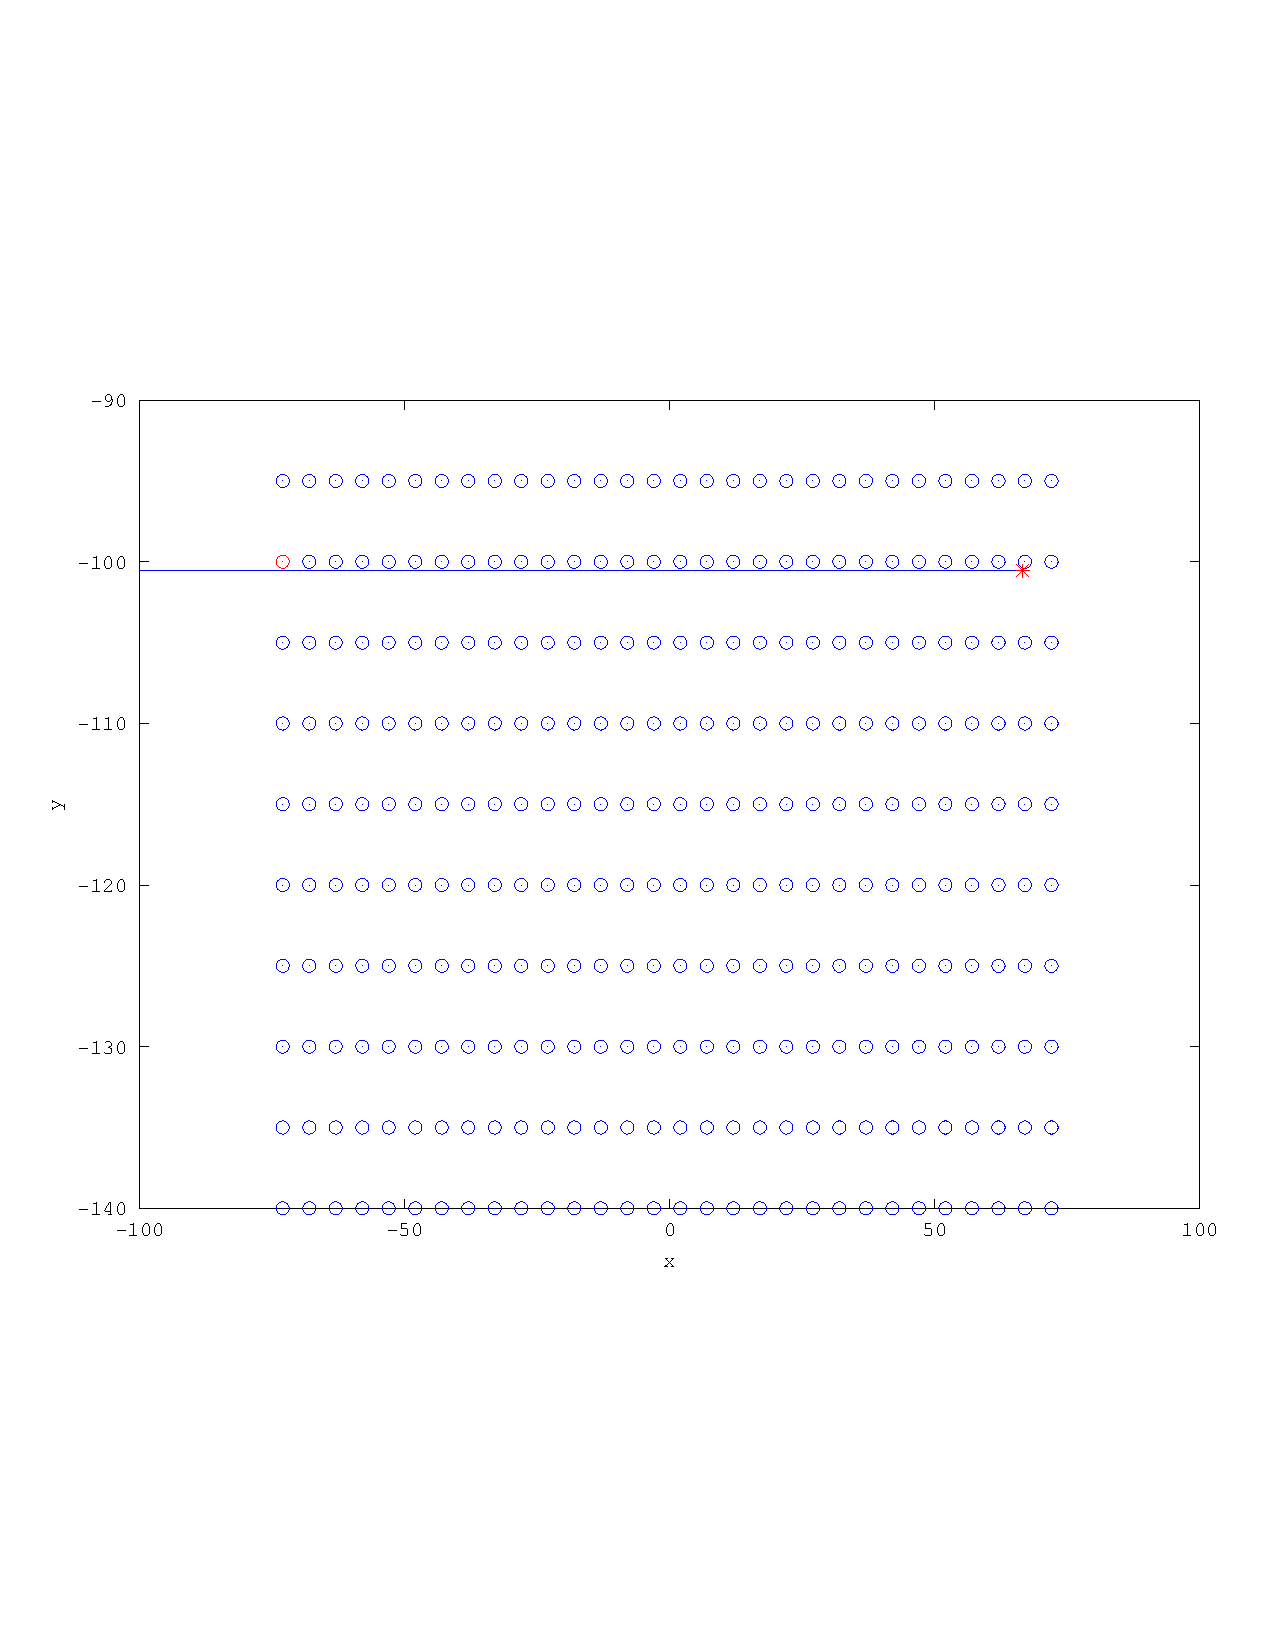
\includegraphics[width=0.6\textwidth]{pics/retract.pdf}
  }
  \caption{Visualization of relevance of all tried retraction point. The red
      point is the finally used point. The red asterisk is the contact point. In
      tis case the ball should be kicked straight forward.
         }
  \label{fig:retraction_plot1}
\end{figure}
\end{frame}

\begin{frame}{Results}
\begin{figure}[htbp]
  \centering
  \makebox[\textwidth] {
    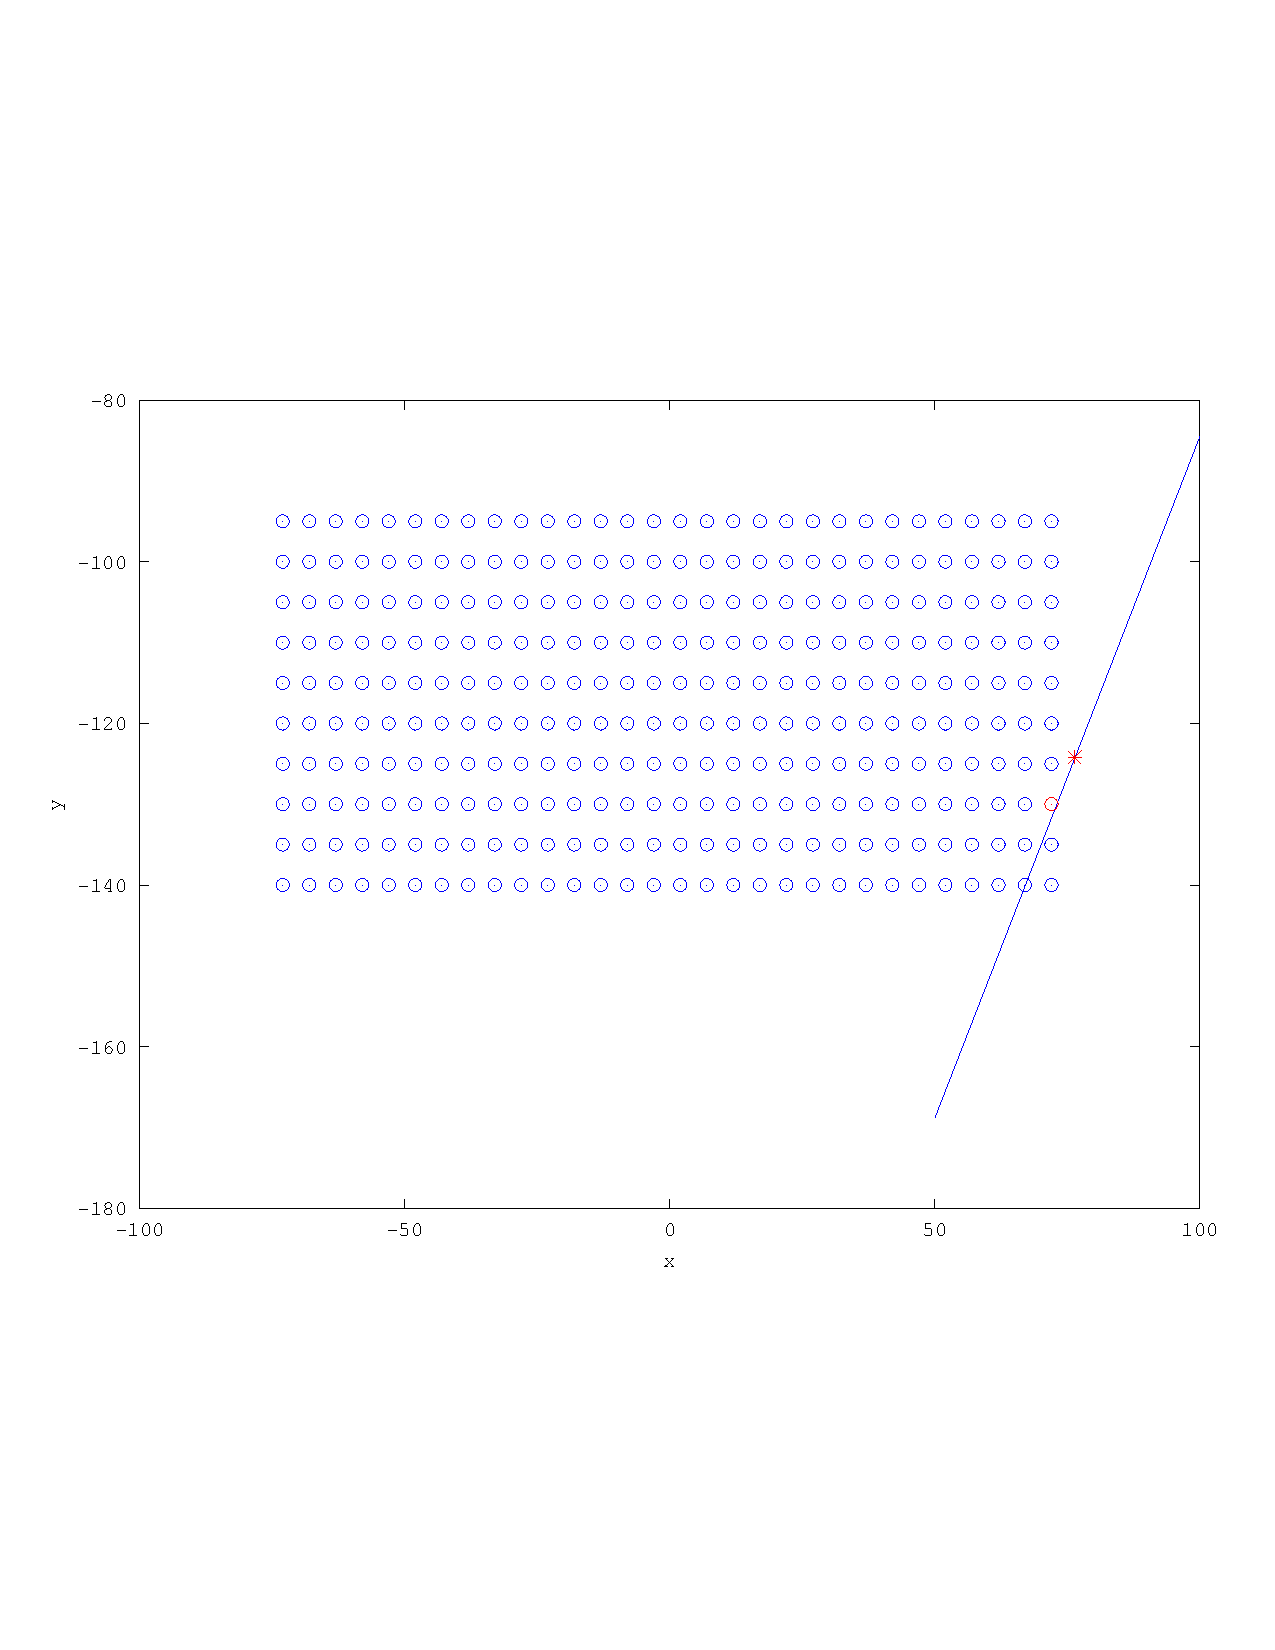
\includegraphics[width=0.6\textwidth]{pics/retract3.pdf}
  }
  \label{fig:retraction_plot2}
\end{figure}
\end{frame}


\begin{frame}{Results}
    \begin{figure}[h]
        \subfigure{
           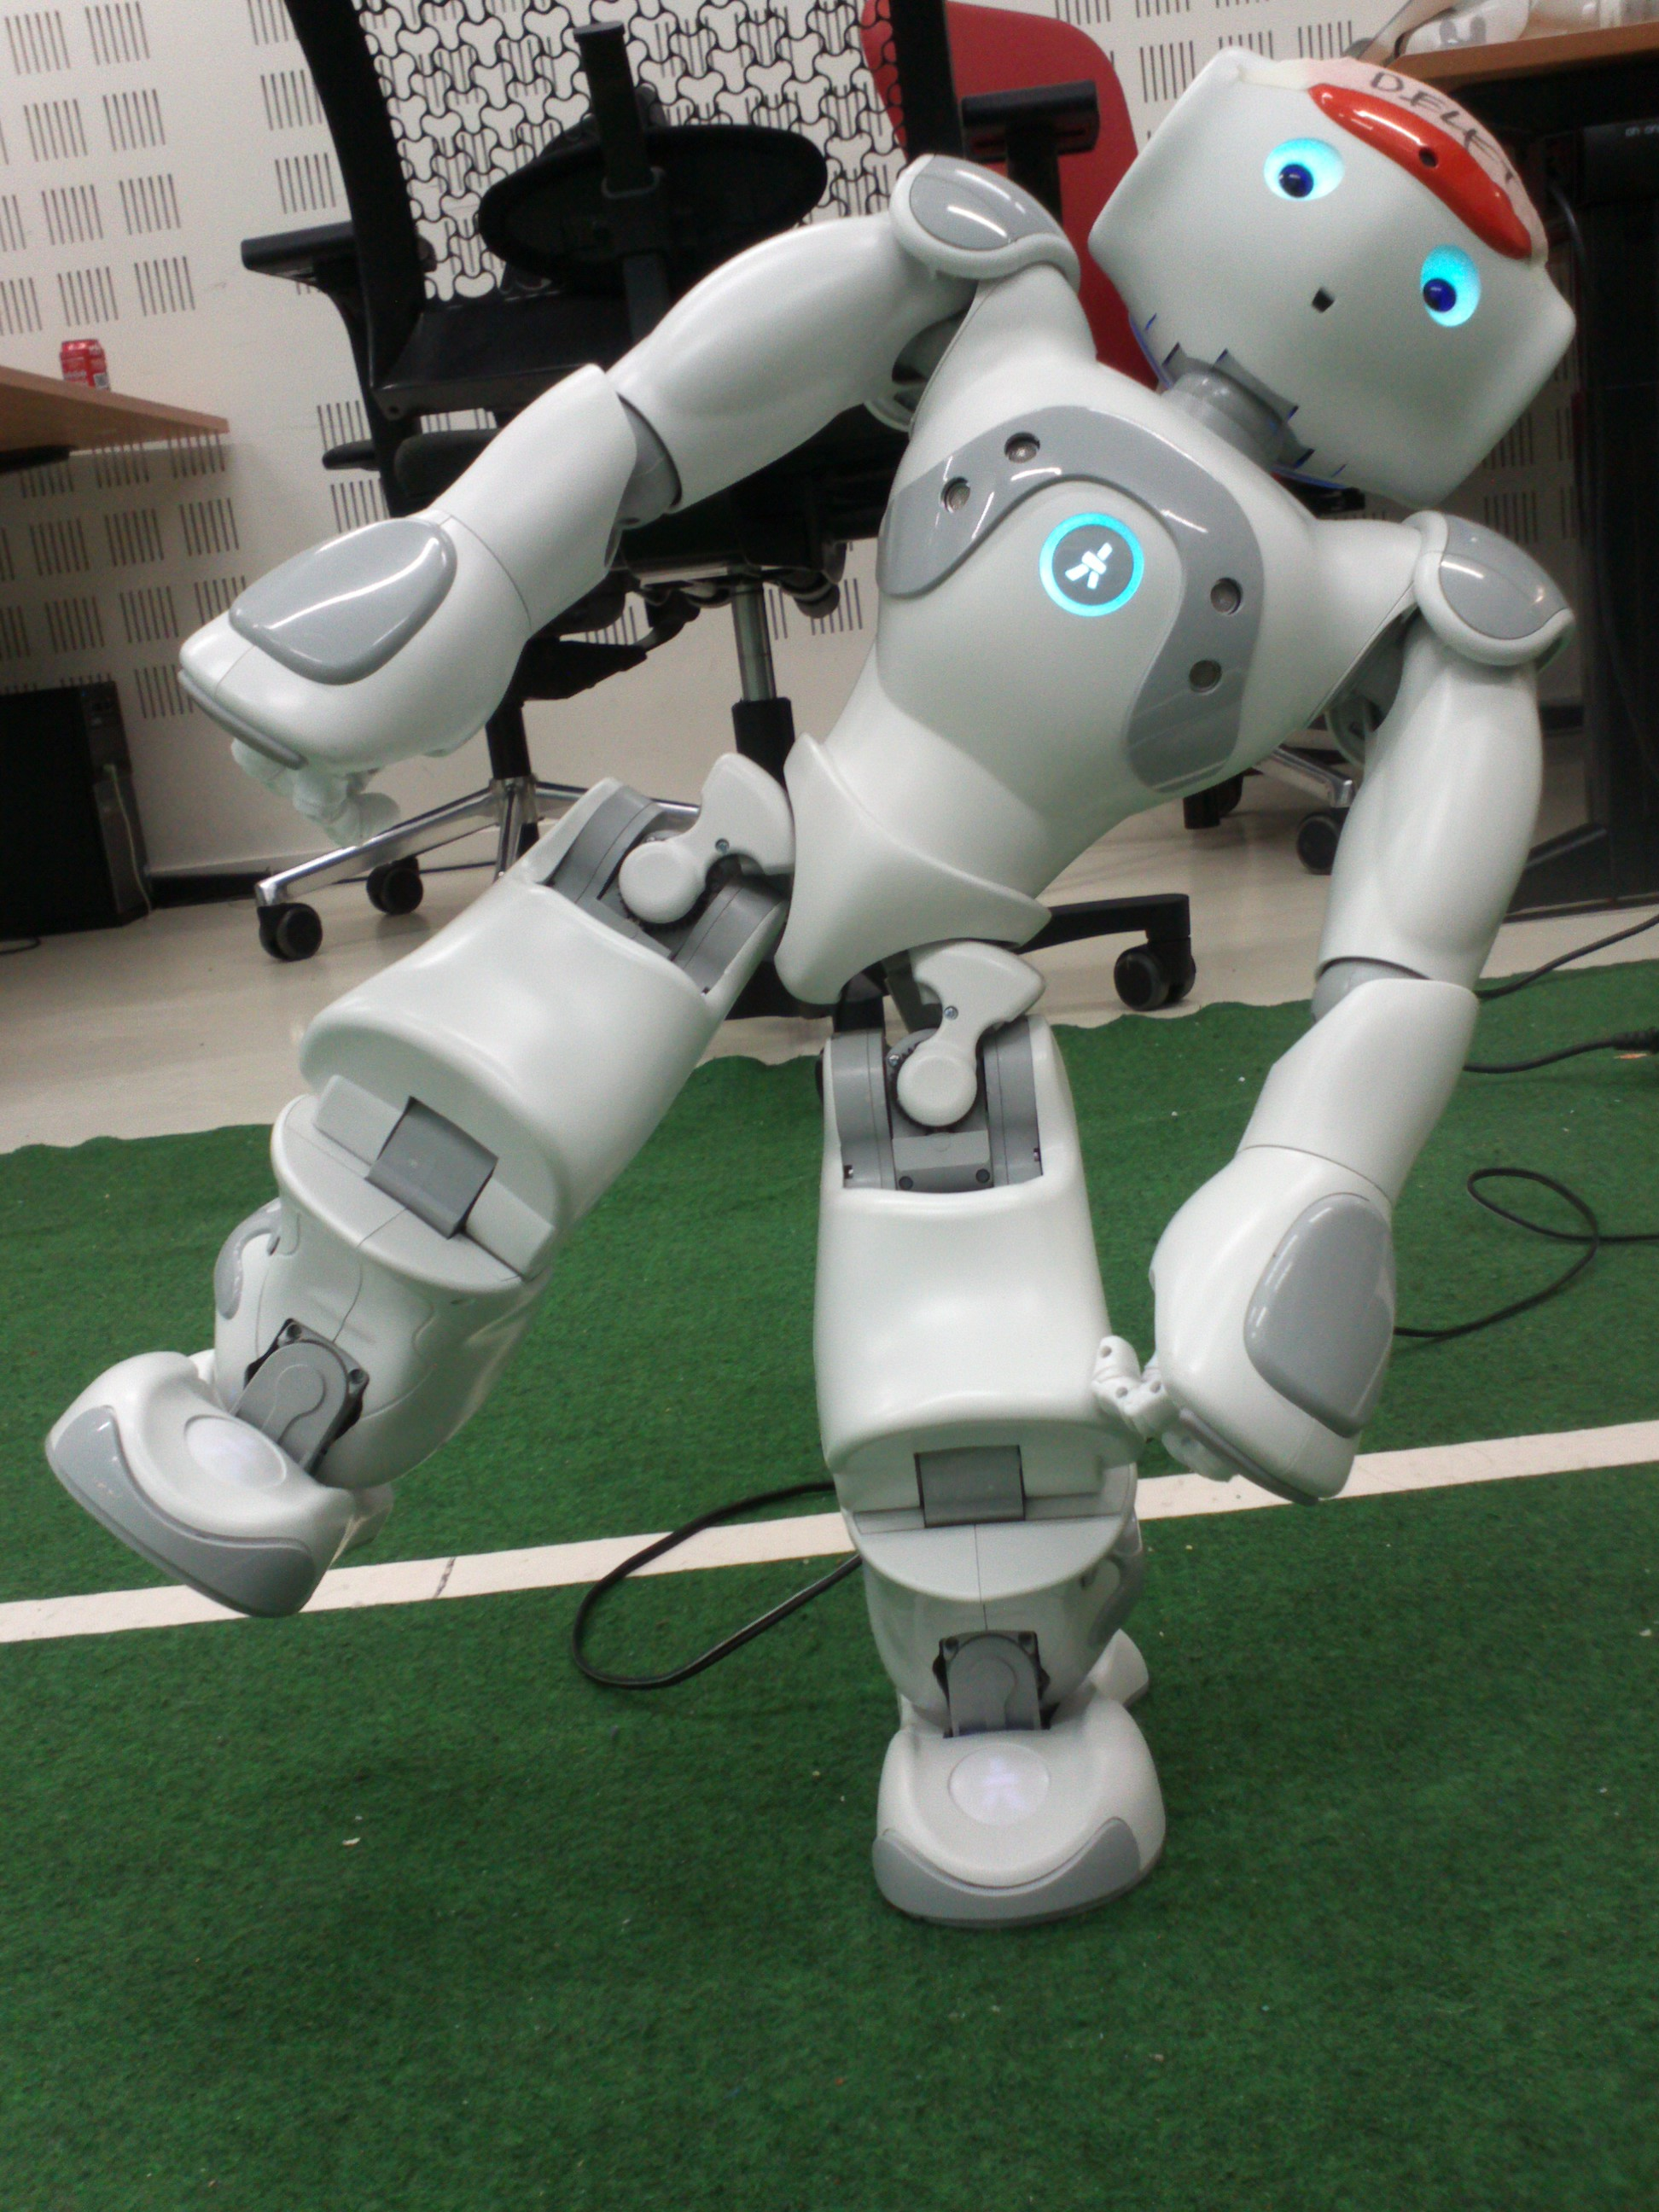
\includegraphics[width = 0.4\textwidth] {pics/nao_initial1.jpg}
         }
         \subfigure{
           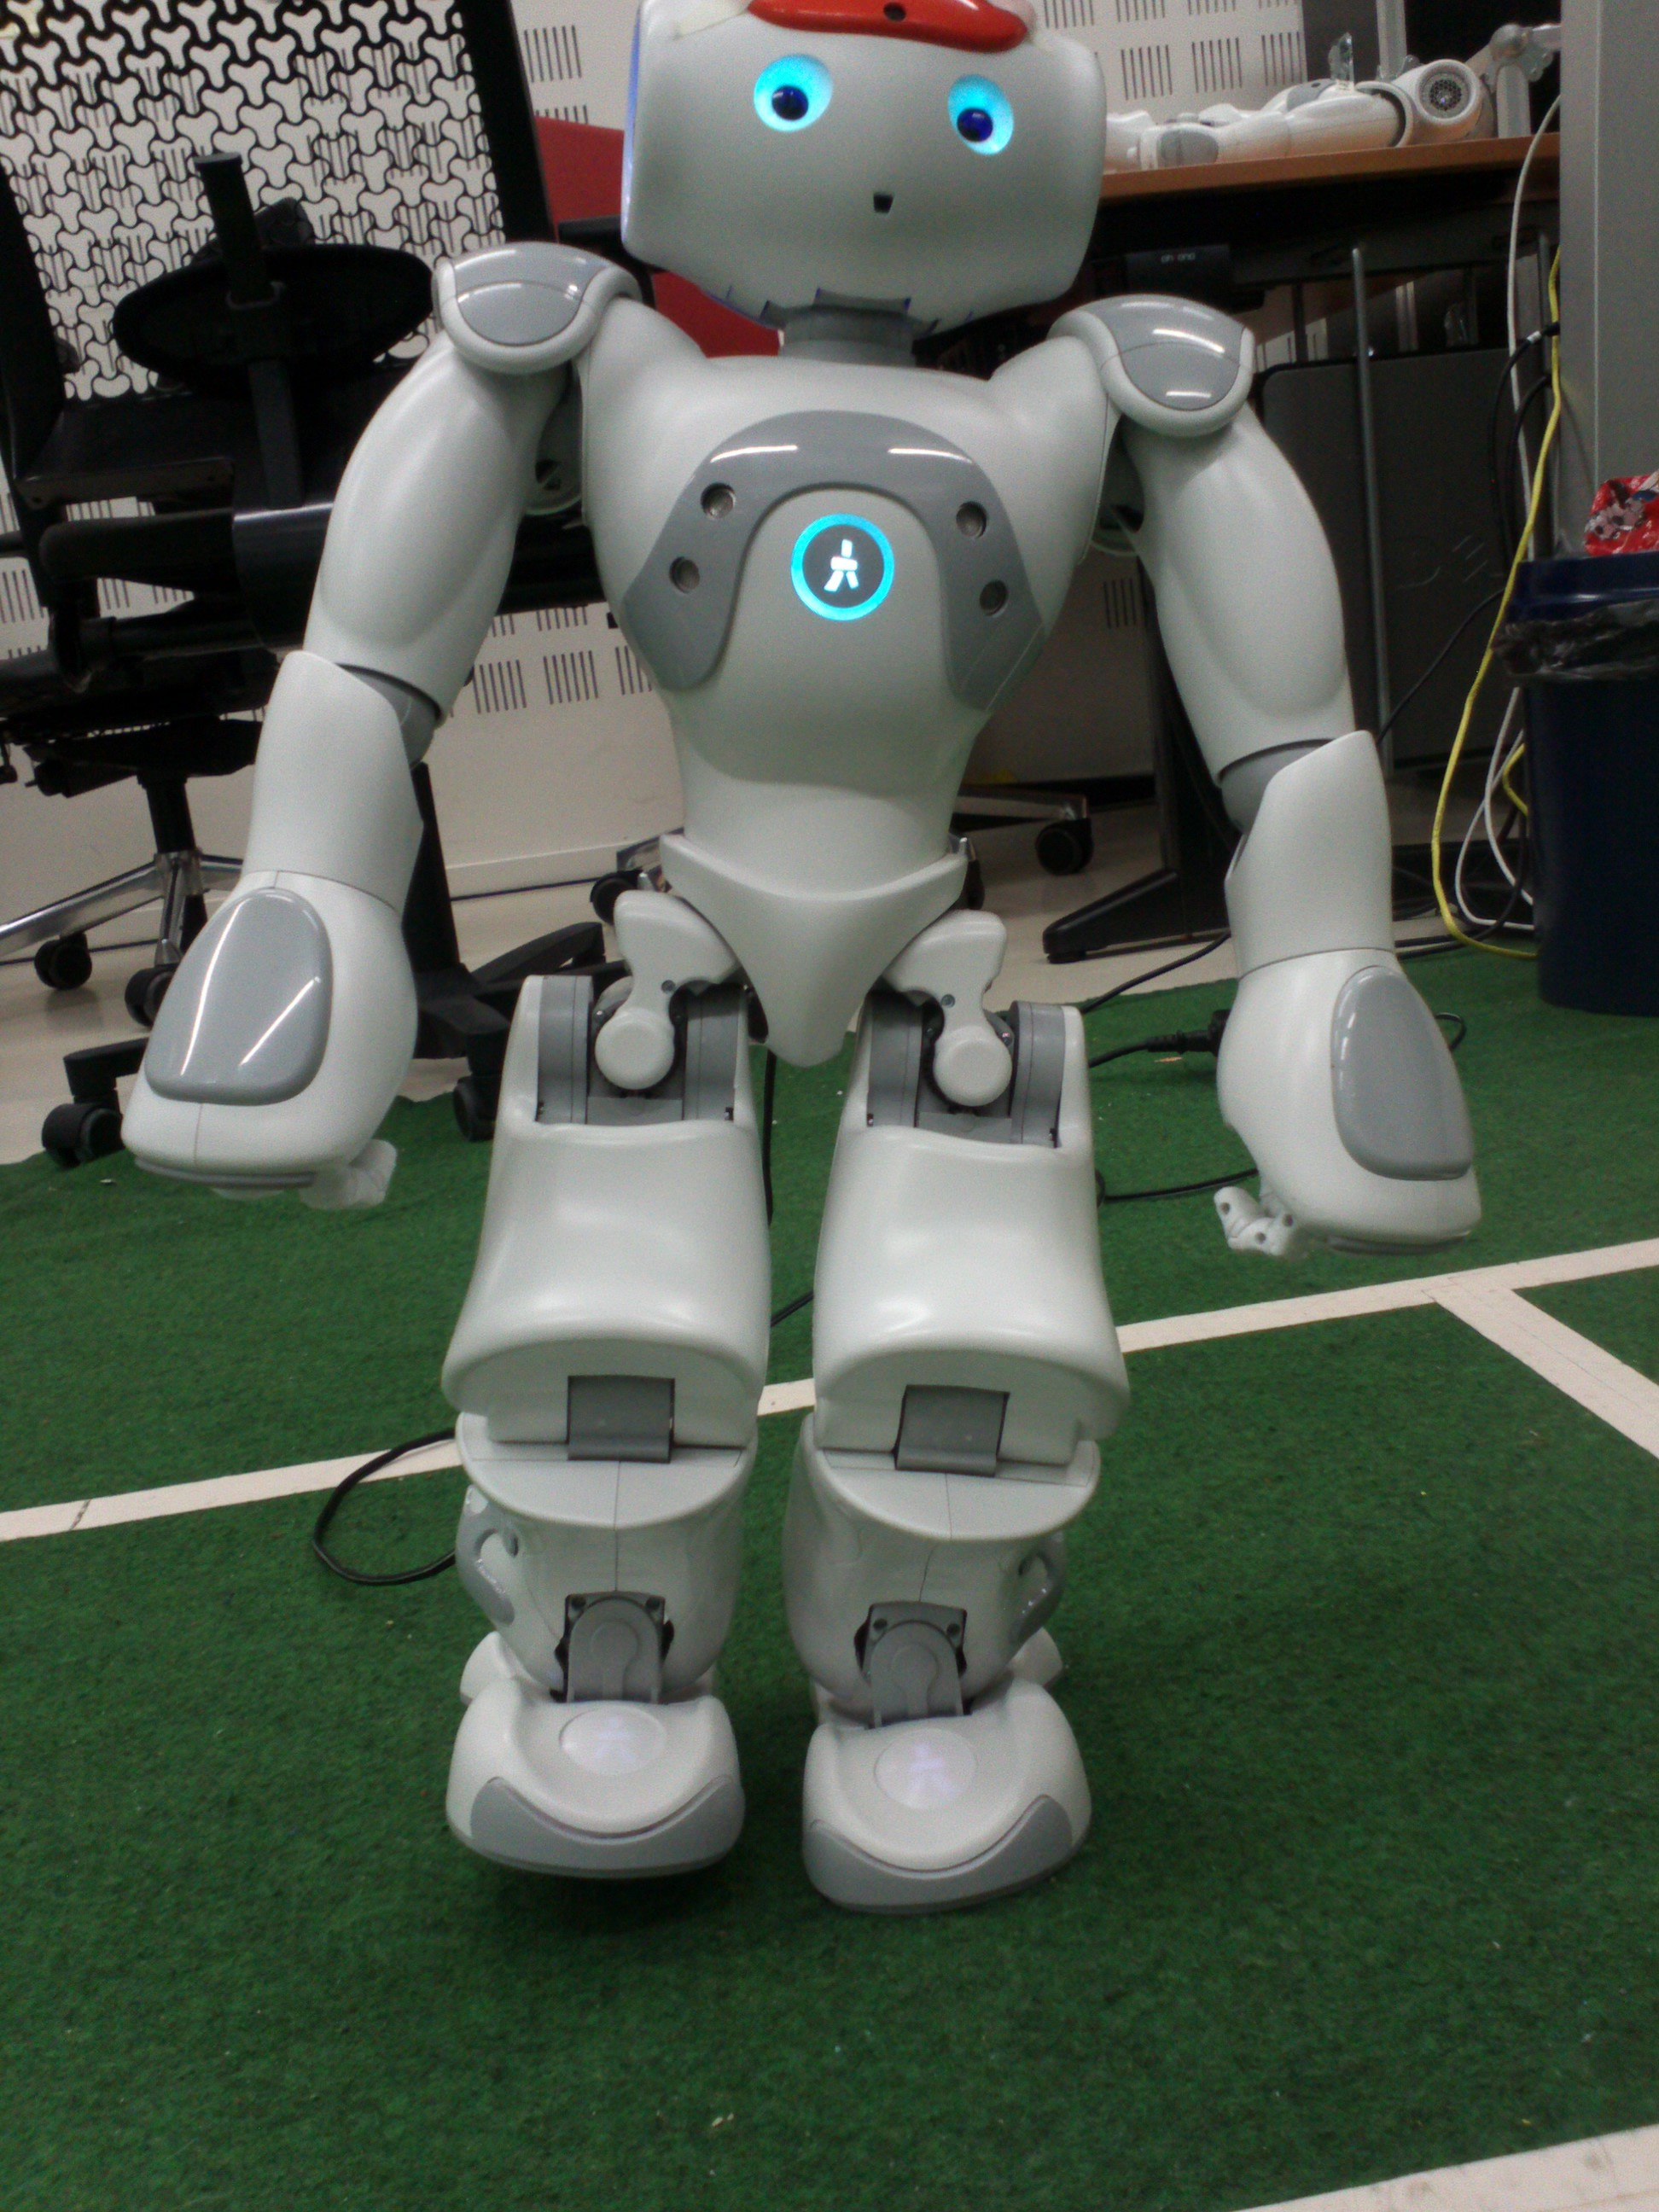
\includegraphics[width = 0.4\textwidth] {pics/nao_initial2.jpg}
         }
    \end{figure}
\end{frame}
\section{Conclusion and future works}

\begin{frame}{Conclusion}
  \begin{itemize}
    \item Individual components are mostly working
    \item Balancing works really well, especially when using the ankle joints
    \item Not enough time to integrate everything into a proper kick
  \end{itemize}
\end{frame}

\begin{frame}{Future works}
  \begin{itemize}
    \item fix the remaining issues
    \item port everything to C++
    \item integrate into Dutch Nao Team code
  \end{itemize}
\end{frame}

\end{document}
